% !TEX encoding = UTF-8 Unicode
% !TEX program = xelatex

\documentclass{article}
	\usepackage[margin = 1.75in]{geometry}
	\usepackage{tikz}
	\usepackage{listings}
	\usepackage{fontspec}
\begin{document}



	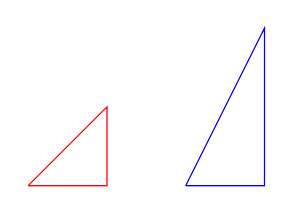
\begin{tikzpicture}
		\draw [red] (0, 0) -- (1, 0) -- (1, 1) -- (0, 0);
		\draw [blue] (2, 0) -- (3, 0) -- (3, 2) -- (2, 0);
	\end{tikzpicture}



	\fontspec{SourceCodePro-Regular}
	\lstset{
		language=[latex]tex, tabsize=4,
		moredelim=*[s][\itshape]{$}{$},
		moredelim=*[s][\color{red!40!.}]{(}{)},
		moredelim=*[s][\color{green!30!.}]{[}{]},
		backgroundcolor=\color{blue!5},
		commentstyle=\color{.!80}\itshape,
		texcsstyle=*\color{blue!40!.},
		moretexcs={
			draw
		},
		deletetexcs={},
	}
	\lstinputlisting{drawcolor.tex}

\end{document}